\documentclass{beamer}

\setbeamertemplate{navigation symbols}{}%remove navigation symbols

\usepackage{tikz}
\usepackage{hyperref}
\usepackage{pgfgantt}
\usetikzlibrary{calc, shapes}

\title{Business Strategy}
\date{}
\author{}

\begin{document}

\frame{\titlepage}

\frame{\frametitle{Project Management}
Make sure things get done when they need to get done. One approach: Gantt Chart.
\pause
\tikzset{every picture/.style={scale=.7}}
\begin{center}
\begin{ganttchart}[hgrid, vgrid]{12}{12}
\gantttitle{Weeks till pitch}{12} \\
\gantttitlelist{1,...,6}{2} \\
\ganttgroup{Code development}{1}{8} \\
\ganttgroup{Code testing}{6}{10} \\
\ganttgroup{Market Research}{1}{4} \\
\ganttgroup{Business Strategy}{1}{5}\\
\ganttgroup{Grand Council Prep}{4}{6}\\
\ganttgroup{Pitch Prep}{6}{12}
\end{ganttchart}
\end{center}

}

\frame{\frametitle{Wingman}

\begin{itemize}
\item \url{http://www.cardiff.ac.uk/racdv/students/Successes/Stuart\%20Jolley.html}
\item \url{http://www.businesszone.co.uk/topic/business-profiles/ones-watch-stuart-jolley-wingman/34554}
\item \url{http://yhponline.com/2011/06/05/stuart-jolley-i-am-wingman-build-the-brand-and-they-will-come/}
\end{itemize}

}

\frame{\frametitle{Million Dollar Homepage}

\url{http://www.milliondollarhomepage.com/}
}

\frame{\frametitle{What is business strategy?}

\pause

\begin{center}
\Large{Convince us that this is not just a cool idea,\\but that it is also a business.}
\end{center}

\pause

2 tools available to help:

\begin{itemize}
\item Swot analysis;
\item Business model canvas.
\end{itemize}

}

\frame{\frametitle{SWOT analysis}
\begin{center}
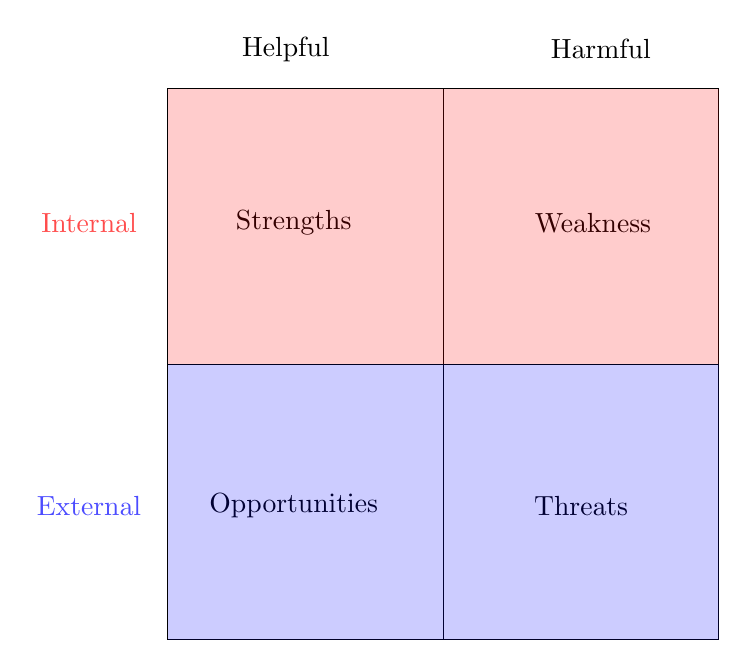
\begin{tikzpicture}
\draw (0,0) rectangle (7,7);
\draw (0,3.5) -- (7,3.5);
\draw (3.5,0) -- (3.5,7);
\node at (1.6,5.3) {Strengths};
\node at (5.4,5.3) {Weakness};
\node at (1.6,1.7) {Opportunities};
\node at (5.25,1.7) {Threats};
\pause
\node at (1.5,7.5) {Helpful};
\node at (5.5,7.5) {Harmful};

\pause
\node at (-1,5.3) [color=red!70] {Internal};
\node at (-1,1.7) [color=blue!70]{External};

\draw [fill=blue,opacity=0.2] (0,0) rectangle (7,3.5);
\draw [fill=red,opacity=0.2] (0,3.5) rectangle (7,7);

\end{tikzpicture}
\end{center}
}

\frame{\frametitle{Business Model Canvas}

\begin{tikzpicture}
\draw (0,0) rectangle (10,-7.071);
\draw (0,0) rectangle (2,-5.071);
\draw (2,0) rectangle (4,-5.071/2);
\draw (2,-5.071/2) rectangle (4,-5.071);
\draw (4,0) rectangle (6,-5.071);
\draw (6,0) rectangle (8,-5.071/2);
\draw (6,-5.071/2) rectangle (8,-5.071);
\draw (8,0) rectangle (10,-5.071);
\draw (5,-5.071) -- (5,-7.071);
\node at (.75,-.25) {\tiny{Key Partners}};
\node at (2.75,-.25) {\tiny{Key Activities}};
\node at (2.75,-5.071/2 - .25) {\tiny{Key Resources}};
\node at (5,-.25) {\tiny{Value Proposition}};
%\node at (7.1,-.5) [text width = 2cm] {\tiny{Customer Relationships}};
\node at (7,-.25) {\tiny{Customer Relations}};
\node at (6.5,-5.071/2 - .25) {\tiny{Channels}};
\node at (9.05,-.25) [text width = 2cm] {\tiny{Customer Segments}};
\node at (.5,-5.071-.25) {\tiny{Costs}};
\node at (6,-5.071-.25) {\tiny{Revenue Streams}};
\end{tikzpicture}

}


\frame{
\frametitle{Links}

\begin{itemize}
\item \url{http://en.wikipedia.org/wiki/Business_Model_Canvas}
\item \url{http://www.businessmodelgeneration.com/}
\item \url{https://www.youtube.com/watch?v=QoAOzMTLP5s}
\item \url{https://www.youtube.com/watch?v=2tdpNKdH7sM}
\item \url{http://en.wikipedia.org/wiki/SWOT_analysis}
\item \url{http://www.youtube.com/watch?v=GNXYI10Po6A}
\item \url{http://www.plainenglish.co.uk/gobbledygook-generator.html}
\end{itemize}
}

\end{document}
